\documentclass[11pt,a4paper]{article}
\usepackage[utf8]{inputenc}
\usepackage{graphicx}
\usepackage{amsmath}
\newcommand{\argmax}[1]{\underset{#1}{\operatorname{arg}\operatorname{max}}\;}
\author{Frank Smit \& Sander Latour}
\title{A game of politics}
\begin{document}
\maketitle

\section{Introduction}
This work introduces and describes the game, `a game of politics'. In this game, the player plays the lead character who invented a super computer which enables him to control the mind of a leader during the prehistoric era. During that time, the power is all divided over different families. These different families have certain ideals and will request the leader for favors which will bring them closer of achieving those. In every turn, the player is able to approve one of these requests. Each request has is own consequences (positive or negative), and will influence the relationship between the families and the leader. 

Credits are assigned to the player after each turn. The goal of the player is to earn as many credit as possible. The amount of credit the player receives is determined by the action he takes. This means that the player should carefully select his actions and think about the consequences it has for his own benefit.  The paper is divided as follows; in the next section the game will be described. In section 3 the implementation details will be discussed and the final sections will be for concluding and discussing this work.

\section{Game}
\subsection{Game mechanics}
The game is a Turn-Based-Strategy (TBS) game, without any time restrictions in each turn. Thus the player has plenty of time to think about the strategy he will play. In every turn their are $N$ actions to choose from (e.g. their are $N$ families are proposing one request). These actions have effects, both negative and positive, to several topics of the world (such as food and safety).  After selecting an action, the agents will immediately react by changing his support and emotion. This will be positively if you consider the ideals of the agent and negatively otherwise. The support of the family towards the player is important to the player because after every turn, the the player needs to satisfy at least 60\% of the people. If the support is below this threshold, the people will stand up to you and will start a revolution. The player then has three turns to get the support back below the threshold else the game will be finished. 

The way the player divides the power could be of great importance for the amount of credit the player receives. For example, the player  could  increase the power of a specific family by favoring him over the others, this will cause people to switch to the winning team and increase the power of the winner. The more people that are represented by one family, the more people you can make happy by approving that family's request. When  a family is completely satisfied with your policy, they could decide to support you unconditionally. This means that they will transfer their power to the player and will not ask for any requests anymore. This support will not be permanently, but will stop once the player disobeys the ideals of the family for a number of turns.

This all means that there are various ways to play the game. The player could try to keep almost everybody happy by giving them all what they want in turn. Or he could try to make one or more actors more powerful and only focus on making them happy. Both methods have upsides and downsides and it depends on the player which one he chooses to achieve the best result.

As mentioned before, the result is measured in credits. The player receives a credit for each turn the people support him. The player could significantly increase his credits by instead of approving one of the actor's desires, decide to spend this turn by giving himself more credits. This will however upset the families, meaning that it can only be successfully applied in specific cases. Once the player is game-over, the credits that were gathered are shown. This creates a motivation to play again to improve your score, and the credits metric also makes the result comparable to strategies of your friends.

%  \begin{itemize}
%    \item The game is turn based, meaning you have plenty of time to think about the next move, and each time you select an action the other actors will respond to that.
%    \item The action space consists of the N requests of N families of which you can select one that you approve each turn. These actions have effects, both negative and positive, to several topics of the world (such as food and safety)
%    \item Each actor will respond positively or negatively depending on the effect of your action on the topics that they find important. At the end of each turn you need to satisfy at least 60\% of the people, so that means you have to focus on balancing relationships in order to make enough people happy each turn.
%    \item You can however increase the power of a specific actor by favoring him over the others, this will cause people to switch to the winning team and increase the power of the winner. The more people that are represented by one actor, the more people you can make happy by approving that actor's request.
%    \item This means there are various ways to play the game. You can try to keep almost everybody happy by giving them all what they want in turn. Or you can try to make one or more actors more powerful and only focus on making them happy. Both methods have upsides and downsides and it depends on the player which one he chooses to achieve the best result.
%    \item The result is measured in credits. You receive a credit for each turn the people support you. You can significantly increase your credits by instead of approving one of the actor's desires decide to spend this turn by giving yourself more credits. This will however upset the actors, so it can only be successfully applied in specific cases. At the end of the game the credits that you've gathered are shown. This creates a motivation to play again to improve your score, and the credits metric also makes the result comparable to strategies of your friends.
%  \end{itemize}
\subsection{Game situations}

  \subsubsection{The winner takes it all}
Every actions in every turn leads to some families that won that round and some families that lost that round. This is determined by calculating how much, trough the families' eyes, the world was made better after selecting that action. In other words, the consequences of the action are weighted according to the ideals of a family. The family that gain the most is considered the winner and the family that gain the least is considered the loser. 

As mentioned above, the families could become more powerful after selecting some actions. This is done using the winner and losers concept, where some amount of power from the  family that lost is transferred to the family that won. This can be seen as people renegade from one family to the other family. The amount of power that is transferred is determined by means of function \ref{func:pt}. 

\begin{align}
y
\label{func:pt}
\end{align}

In the case of multiple winning and multiple losing families, the most powerful family that won will receive power from the most powerful family that lost. 

\subsubsection{Revolution}
As shortly mentioned before, once the player does not get the 60\% support that is necessary , the families will start a revolution. The player then has three turns to get back the 60\% support that he needs, else the game will be finished. In this situation the families are angry and therefore will ask more of the player then usual. This will make it more difficult, but not impossible, for the player to take everyone's ideals in consideration. The player really has to think of his strategy to avoid losing the game.

\subsubsection{Retirement}
After 67 turns, the leader will decide to retire from his function. Once this happens the player have lead the leader to a successful reign and will be rewarded for his service record. This reward will be in terms of extra credits. 

\subsection{Music}
Music is added to the game to enhance the gaming experience. There are two different states in the game that alters the music. The first one is the normal situation where the player is just picking actions and the agents are reacting to the actions. The second one is when the support is below the threshold of 60\%, i.e. when the revolution starts. The music then is changed to a more tension increasing piece of music. This will create more excitement for the player, knowing that he will need to watch his steps. 

\section{Implementation details}
  \subsection{World state}
    Actions that are performed have an effect on the world. These effects are in turn used by other agents to determine their reaction on the performed action. Since actions can have both positive and negative effects they can reverse some of the earlier actions taken in terms of the world state. To avoid the enormous complexity of a set of boolean variables to represent the diversity of actions and cater for the reversal effect like one would in a classical STRIPS approach, we instead chose to represent the world in a $n$-dimensional space of $n$ real-valued topics. These topics represent typical themes that have been playing a role in politics for a long time. The topics that we have used for the current implementation are \emph{food}, \emph{safety} and \emph{culture}. This list is however extendable. Each world state consist of $n$ topic-value pairs representing the current state of each topic in that world state.
  \subsection{Actions}
    Not unlike STRIPS actions consist of two parts, a condition and the effect. These two components are described in terms of the topic space as was discussed earlier.
    \subsubsection{Conditions}
      Each action has a set of topic-value pairs that represents the minimum value that each mentioned topic must have in the world state before the action is requested. This is motivated by the following reasoning. If an agent values a specific topic it will naturally try to improve that topic as much as possible. However if the basic necessities of a topic are not arranged yet, it has no use to request higher level improvements since they typically rely on the presence of more basic improvements for their effectiveness. The topic values for consecutive actions are increasing. The condition also has the effect that when another action decreases a topic value, it might result in some agent requesting earlier actions again.
    \subsubsection{Effects}
      Each action has a set of topic-value pairs that represents the effect it has on the world state. The values can be both positive and negative indicating positive and negative effects respectively. The new world state can be determined by simply adding each of the effect values to the current world state values.
  \subsection{Autonomous agents}
    Most players in the game are autonomous agents that each turn determine which action they would most desire to see executed by the human player. This desire is expressed to the human player at the beginning of each turn. When a human player decides which action to execute, each autonomous agent will determine his reaction to this action. The reaction is a positive or negative change in their emotional state.
    \subsubsection{Selecting desired action}
      Each agent selects their next desired action according to the following list of steps.
      \begin{enumerate}
        \item Let $\vec{s}$ denote a real-valued vector, where each element denotes the value of a topic in the current world state.
        \item Let $a$ denote an action, consisting of a condition component denoted as $a_C$ and an effect component denoted as $a_E$.
        \item Let $\mathcal{A}$ denote the set of all actions, such that for each valid action $a$ it holds that $a \in \mathcal{A}$.
        \item Let \textsc{Performable}($a_C$,$\vec{s}$) denote a boolean function that returns true when every condition in $a_C$ is met in world state $\vec{s}$.
        \item Let $\mathcal{P}$ denote the set \{\textsc{Performable}($x$)$\vert x \in \mathcal{A}$\}.
        \item Let $\vec{w}$ denote a real-valued vector, where each element denotes the weight of a topic in the world state indicating the preference of the agent.

        \item Return $\argmax{a \in \mathcal{P}} \left[ a_E \cdot \vec{w} \right]$.
      \end{enumerate}
    \subsubsection{Preferences}
      Each autonomous agent prefers improvement in some topics more than in others. It might even prefer to worsen the situation of a specific topic. This is expressed in the preferences, which is a set of topic-weight pairs where the weights adds up to 1. These weights indicate how much they value improvement on that topic.
    \subsubsection{Emotion states}
      Each autonomous agent has a certain amount of emotional energy. This energy is increased when the agent is more pleased. After each turn agents update their emotional energy by summing up the multiplication of the preference weights with the effects of the taken action, which results in the delta value that is added to the current emotional energy level. The continuous domain of the energy is discretized in a FSM of emotional states. The transitions in this FSM are absolute energy values that the agent must be in to switch to a different emotion state. For example, given a sufficiently large negative value an agent will transition from a neutral to an anger state. The current implementation does not use these emotion states very extensively, besides using them to make the energy values more intuitive to understand for the human player. However, they cater for complex behaviour where each agent may behave differently in a different emotion state.
  \subsection{Human agent}
    \subsubsection{Interface}
      The interface of the game, as shown by figure \ref{fig:scr}, is extremely simple and intuitive. Because the story of the game allows the player to play as a scientist who created a super computer, the only screen the player will look at is a computer screen. This screen contains three areas. The first area is the largest one, where the agents together with their request and the consequences are presented. At each line the player has the ability to press the `Approve request' button. This button represents the action the player could take. 

      In the small area left below in the screen, the game information is presented to the player. Here information such as, in which turn the player is, how much credits it received so far, and how much support the player has from the agents. This information will be updated after every turn. In the small area in the right corner below, the world state is presented to the player. This shows the current values of the topics that together form the world state. These topics are the same as the consequences of each action. 

      \begin{figure}[h!]
      \centering
      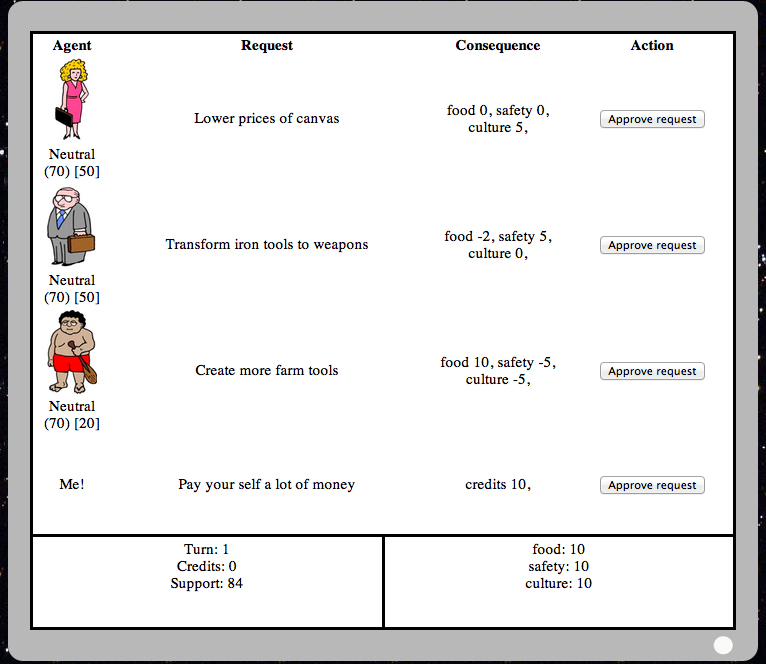
\includegraphics[scale=0.5]{screenshot}
      \caption{A screenshot of the game. The interface is simple and intuitive, having different screens containing different sort of information. }
      \label{fig:scr}
      \end{figure}
  \subsection{Game loop} 
  (explain image)
    \subsubsection{Collect desires}
    \subsubsection{Request approval}
    \subsubsection{Execute action}
    \subsubsection{Inform agents}


\section{Conclusion}
A game of politics can be considered as a serious game that simulates a part of the decision making process of leaders in a small domain. 

 
  \begin{itemize}
    \item Created a serious game that simulated a part of the decision making process of leaders
    \item Up to a certain point managed to achieve multiple winning strategies
  \end{itemize}
  
\section{Discussion}
  \begin{itemize}
    \item Turned out to be difficult to balance realism and what is doable in practise.
    \item Turned out to be difficult to create good gameplay with various factors that complicate behavior (how to keep it surprising but understandable)
    \item Turned out to be difficult to create a good story and good actions that make it more realistic and interesting.
    \item Turned out to be difficult to create the game in such a way that it is not biased to any of the strategies
    \item Frank, jij had toch nog iets bedacht?
  \end{itemize}
\end{document}
